\section{Towards Tighter Upper Bounds with Top-K Lists}
\label{sec:TighterBounds}

%Upper bounds are attractive for query optimization because they provide robustness: By preparing the query execution plan for the worst possible scenario, the database system can never produce overly optimistic plans that lead to catastrophic regressions. If however the calculated upper bounds overestimate the actual cardinalities by a large margin, plans may become too defensive and refrain from using operators and join orders that work best on small amounts of tuples. This in turn may lead to slower queries. To circumvent this issue, we explore means to tighten the UES upper bounds while still relying on basic table statistics.

As presented in the previous section, \emph{PostBOUND} is a novel framework for upper bound-driven query optimization of SPJ queries based on a generalized version of the UES concept~\cite{hertzschuch-21-ues}. 
Since the original UES algorithm only calculates upper bounds based on the most frequent attribute value~\cite{hertzschuch-21-ues}, this upper bound approach highly overestimates the join intermediate cardinalities (cf. Fig~\ref{fig:UESOverestimationJOB}) leading to a very defensive approach and refrains from using physical join operators and join orders that work best on small amounts of join tuples. 
To overcome that and to demonstrate the extensibility of \emph{PostBOUND}, we introduce two tighter upper bound variant ideas in this section. 

A natural extension of the UES upper bound is to consider not only the largest attribute value frequency, but the largest $k$ frequencies along with their corresponding attribute values. 
Such information is typically stored in \emph{top-k} lists (sometimes also called \emph{most frequent values}), which basically are an ordered sequence $((v_1, f_1), ..., (v_k, f_k))$ of attribute values $v_i$ and their corresponding frequencies (i.e. number of occurrences) $f_i$, such that $v_1$ is the most frequent value, $v_2$ the second most frequent value, and so on.
Such a top-k list can be used for two basic purposes: for all attribute values that are present in the top-k list of both join partners, their frequency can be used directly to calculate the number of outgoing tuples for a join. 
For all attribute values that are not contained in the top-k list, their maximum frequency can still be derived based on the minimum frequency in the list, i.e. the $f_k$ frequency: If the frequency were higher, the attribute value would be present in the top-k list in the first place.

Based on these top-k lists, we devise two basic families of algorithms to calculate an upper bound for a join \sql{R.a = S.b}: The \emph{first family} divides both \sql{R.a} and \sql{S.b} into two disjunct sets, one that encompasses all attributes that are contained in the respective top-k list, and one that contains the remaining values. 
For all values that are in either top-k list, the number of tuples in the join result can be calculated accurately. 
For all values that are in neither top-k list, a fallback strategy is used. 
The \emph{second family} calculates the upper bound by simulating a worst-case join scenario. 
This is achieved by iteratively joining attribute values from the top-k lists, such that the overall cardinality is maximized. 
This strategy directly adopts the pessimistic nature of UES in that it considers the absolute worst case distributions of attribute values for both \sql{R.a} and \sql{S.b}.

In the remainder of this section, we present two examplary algorithms from both families, starting with the \emph{approximate top-k bound} as an instance of the first family, followed by the \emph{cautious top-k bound} from the second family. 
These formulas are not the only instances of their respective families and they are by no means perfect. 
Instead, they serve as a starting point for further research. 
The section concludes with some remarks regarding the update of top-k lists when considering $n$-way joins. 
To keep notation short, we use the following definitions: we calculate an upper bound for a join \sql{R.a = S.b} between attributes $R.a = (a_1, a_2, ..., a_n)$ and $S.b = (b_1, b_2, ..., b_m)$. 
As long as there is no ambiguity, we refer to each attribute by its relation, e.g. instead of $R.a$ we simply write $R$. 
$|R|$ and $|S|$ denote the number of tuples in each relation. 
Both attribute sets have an associated top-k list $\text{top}_R \subseteq R.a$ and $\text{top}_S \subseteq S.b$. 
For each attribute value $x$, we define the \emph{attribute value frequency} as follows:

\begin{equation*}
    AF_R(x) \coloneqq
    \begin{cases}
    |\{a \in R\;|\;a = x\}| & \text{if $x \in \text{top}_R$} \\
    f^\ast_R & \text{otherwise}
    \end{cases}
\end{equation*}

$f^\ast_R$ denotes the minimum frequency of any value in the top-k list of $R$. 

\subsection{Approximate Top-k Bound}
\label{sec:tighter-bounds-approximate}

The main idea of the \emph{approximate bound} is to split the calculation into two parts, i.e. $\text{upper}(R.a = S.b) \coloneqq \text{upper}_\text{top}(R.a = S.b) + \text{upper}_\text{rem}(R.a = S.b)$, where the first bound is directly based on the top-k lists and the second bound accounts for all remaining attribute values. 
Deriving an upper bound for values in the top-k lists is pretty straightforward: for each value in either top-k list, its frequency is multiplied by the value frequency in the other top-k list, falling back to $f^\ast$ if necessary. 
Thus, $\text{upper}_\text{top}$ can be expressed as

\begin{definition}[Top-k based approximate upper bound]
    \begin{equation}
        \text{upper}_\text{top}(R.a = S.b) \coloneqq \sum_{a \in R.a} AF_R(a) * AF_S(a)\:+\sum_{b \in S.b \setminus R.a} AF_R(b) * AF_S(b)
    \end{equation}
    \label{def:approx-bound-topk}
\end{definition}

\begin{figure}[tb]
	\centering
	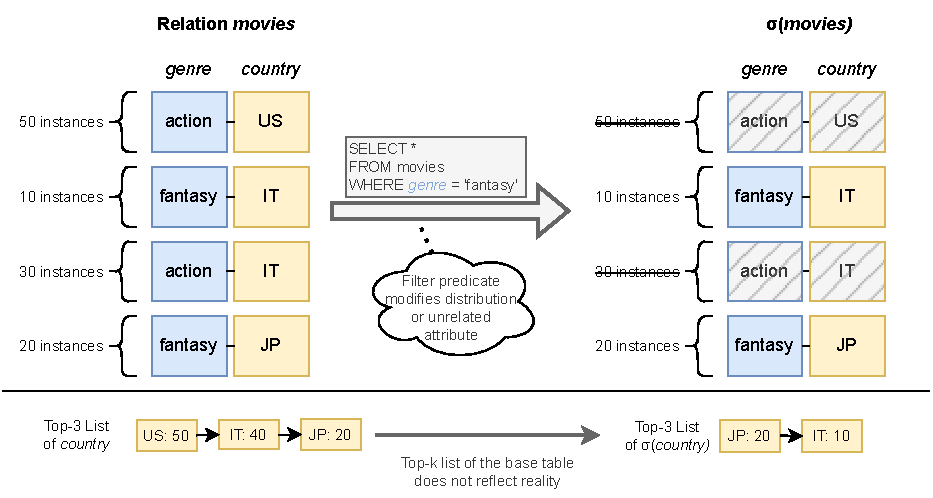
\includegraphics[width=\linewidth]{figures/topk-filters.pdf}
	\caption{Static top-k lists can be misleading due to filter predicates.}
	\label{fig:topk-filter-mismatch}
	\vspace{-0.4cm}
\end{figure}

Deriving an upper bound for all remaining attribute values is significantly harder: Although in principle the UES formula can be used to estimate the maximum cardinality of two attribute sets based on their maximum frequency, some of these values might have already been processed as part of $\text{upper}_\text{top}$. 
Thus, these values should not be considered again in the remaining bound. 
This strategy suffers from a fundamental disconnect between the top-k list of an attribute \sql{R.a} and the attribute instances that are actually available: top-k lists are computed for all attribute values in a base table. 
However, at query runtime, the distribution and count of these attribute value instances may be changed fundamentally after applying filter predicates on the base tables. 
Consider Fig.~\ref{fig:topk-filter-mismatch}: the filter predicate completely removes the most frequent value and changes the order of the remaining two attribute values. 
Since the filter predicate can be entirely independent from the attribute being joined, the top-k list can only be considered a static upper bound of the true attribute frequencies.
Since there is no direct way to determine which attribute instances are actually available after executing the filter predicate as long as only basic statistics are considered, we make the pessimistic assumption that none of the values from the top-k list are actually available.
Thus, the $\text{upper}_\text{rem}$ becomes a full UES bound based on the maximum remaining frequency, i.e. $f^\ast$:

\begin{definition}[Remaining UES bound of the approximate top-k bound]
    \begin{equation}
        \text{upper}_\text{rem}(R.a = S.b) \coloneqq \min \biggl( \frac{|\sigma(R)|}{f^\ast_R}, \frac{|\sigma(S)|}{f^\ast_S} \biggr) * f^\ast_R * f^\ast_S
    \end{equation}
    \label{def:approx-bound-remainder}
\end{definition}

The issue of top-k lists that are unrelated to the attribute instances is actually also present when calculating the $\text{upper}_\text{top}$ bound: the processed frequencies can significantly overestimate the number of tuples that are truly available. 
However, in this case, we know the total number of available tuples as well as the number of processed tuples per relation. 
Thus, we can slightly mitigate the impact of overestimation by constructing an adjustment factor for \sql{R} as well as for \sql{S}. 
Each factor is simply the ratio between available tuples and processed tuples. 
The factors will be applied as soon as they are smaller than 1 (i.e. there was an overestimation). 
Strictly speaking, this trick assumes a uniform distribution of the overestimation, i.e. each attribute value is overestimated by the same fixed delta. 
This may drop the upper bound for the top-k list below the actual cardinality in some rare cases. 
By applying the $\text{upper}_\text{rem}$ bound as defensively as presented in Definition~\ref{def:approx-bound-remainder}, this issue is largely mitigated, leaving the bound \emph{effectively} as an upper bound. 
Still, there may be situations where the overestimation via $\text{upper}_\text{rem}$ is not enough to compensate the underestimation caused by the adjustment factors, hence the name of an \emph{approximate} upper bound.

\subsection{Cautious Top-k Bound}
\label{sec:tighter-bounds-cautious}

The approximate nature of the previous bound motivates research in an entirely different direction. 
The \emph{cautious top-k bound} iteratively tries to construct the maximum number of join tuples based on the entries in the top-k lists and the total number of available tuples. A pseudo-code implementation of this strategy is given in Algorithm~\ref{alg:cautious-topk-bound}:

\begin{algorithm}[tb]
    \caption{Pseudo-code implementation of the cautious top-k bound.}
    \label{alg:cautious-topk-bound}
    \begin{algorithmic}[1]
        \Function{cautious bound}{top(R), top(S), |R|, |S|, current bound}
            \If{|R| = 0 or |S| = 0}
                \State \Return current bound
            \EndIf
            \If{top(R) is empty and top(S) is empty}
                \State calculate UES bound based on $f^*$ and remaining tuples counts
                \State \Return current bound + UES bound
            \EndIf
            \ForAll{attribute values $v$ in top(R) and top(S)}
                \State $candidate \gets AF_R(v) * AF_S(v)$
                \State $|R'| \gets max(|R| - AF_R(v), 0)$ \Comment adjust the remaining tuples
                \State $|S'| \gets max(|S| - AF_S(v), 0)$
                \State limit top(R') frequencies and $f^\ast_R$ to |R'| \Comment top(R') $\coloneqq$ top(R) $\setminus\:v$
                \State limit top(S') frequencies and $f^\ast_S$ to |S'| \Comment $f_i' = min(f_i, |R'|)$
                \State value bound $\gets candidate\:+\:$ cautious bound(top(R'), topk(S'), |R'|, |S'|) 
            \EndFor
            \State \Return current bound + maximum value bound
        \EndFunction
    \end{algorithmic}
\end{algorithm}

In each iteration, the cautious top-k bound tries to obtain the maximum possible bound given its current state. 
This is achieved by systematically simulating the number of outgoing tuples for each attribute value in the top-k lists. 
For each value, the size of its partial join result is calculated (line 8) and included in the upper bound. 
Afterwards, the top-k lists as well as the total number of available tuples are adjusted based on the value that was just ``consumed'' (lines 9 to 12). 
To adjust the total number of tuples available for each relation, the value's frequency is simply subtracted from the current count. 
Top-k lists are updated to no longer include the candidate value and each frequency including $f^\ast$ is enforced to be at most as large as the remaining number of tuples. 
At this point, the maximum bound for the smaller top-k lists can be calculated (line 13), leading to a recursive structure. 
Recursion terminates if either no more tuples are available (line 2), or the top-k lists are empty (line 4). 
In the first case, both relations have been consumed completely and the current bound is the maximum bound for this branch. 
In the second case, the remaining values are estimated using the UES bound. 
Once the bound for all candidate values has been determined, the algorithm selects the maximum possible bound and calculates the final bound (line 14).

This strategy effectively determines the upper bound for each permutation of attribute value instances and thus suffers from a large computational complexity if implemented naively. 
However, a more elaborate implementation can effectively reuse large parts of the computation and also terminate the bound estimation early if no improvement above the current maximum bound is possible.
Such optimization techniques for an efficient implementation should be explored in future research. 

\subsection{Updating Top-k Based Statistics for $n$-way Joins}
\label{sec:tighter-bounds-stats}

\begin{figure}[tb]
	\centering
	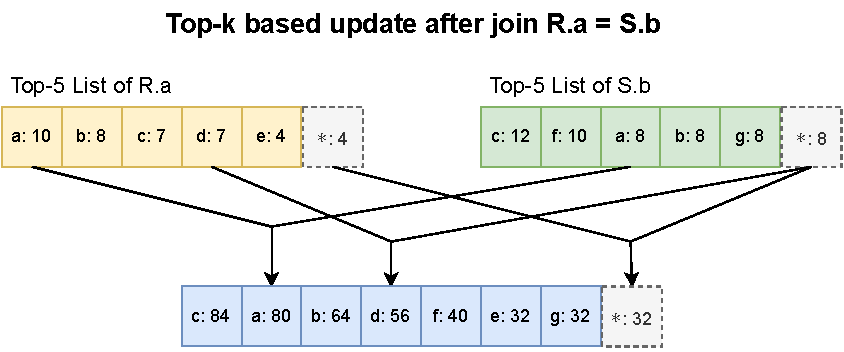
\includegraphics[width=0.8\linewidth]{figures/top-k-update.pdf}
	\caption{Merging two top-k lists after a join.}
	\label{fig:topk-update-merge}
	\vspace{-0.4cm}
\end{figure}

Besides the calculation of the upper bounds themselves, the underlying data structures also have to be updated to estimate higher-order joins that involve 3 or more relations. 
In the case of top-k lists, this issue is twofold: First, the top-k lists of the join attributes have to be combined, integrating the knowledge of both individual lists. 
This problem can be solved in a straightforward manner: The resulting top-k list contains the sum of both source frequencies for each value in either top-k list, again falling back to the $f^\ast$ frequencies as necessary (Figure~\ref{fig:topk-update-merge}). 
The $f^\ast$ frequency of the merged top-k list can likewise be estimated as the product of both source $f^\ast$ frequencies. 
The second case is the update of a top-k list that is not directly involved in the join (a \emph{third-party list}). 
This process is especially important since that list may take part in a later join and the associated frequencies must therefore reflect the current state of the intermediate join result. 
The fundamental problem for this update is the lack of correlation information between the joined top-k list and the third-party list. 
For an upper bound-driven approach, this demands another pessimistic assumption: In the worst case, each entry in the third-party list could correlate entirely with the maximum frequency of the joined top-k list. 
Thus, the maximum possible frequency of each updated value in the third-party list is the product of its current frequency and the maximum frequency in the joined top-k list. 
In general, this strategy will heavily overestimate the frequencies in the updated top-k list, but without additional information or simplifying assumptions it is not possible to figure out how much each frequency has been overestimated. 
This matches the basic maximum frequency update of UES and generalizes that idea to top-k lists.
